

\subsection{Datasets} 
\label{sec:datasets} 

AMI corpus and ICSI corpus are publicly available datasets that contain 100 hours and 70 hours of meeting conversations recorded respectively. The duration of the audio files is between 20 minutes to 1 hour and 30 mins and there are 169 files in total. All the files are in
.wav format. The audio files consist of recording of multiple speakers interacting in workplace meeting.


AMI Corpus \cite{AMIurl, kraaij2005ami}, Augmented Multi-party Interaction Project, funded by the European Commission. 
ICSI Corpus \cite{ICSIurl, janin2003icsi}, International Computer Science Institute Speech Group, UC Berkley.
Reference Summary - Yale-LILY/QMSum: Dataset for NAACL 2021 paper: "QMSum: A New Benchmark for Query-based Multi-domain Meeting Summarization" (github.com)

We are also using reference summaries to train the model. The reference summaries are made by humans for the same meetings found in the AMI and ICSI corpus and are in text-format. The summaries are around a paragraph in length with 80 to 150 words.


\subsubsection{Data Preprocessing}

The audio files are relatively clean but quite lengthy, each conversation is around 50 mins long. One difficulty that we are facing is the length of the audio files. We are relying on OpenAI’s Whisper to transcribe the audio files and also using pyannote to diarize the sudio before combine the two to create the complete transcript. We used 1-GPU for carrying out the processing on the audio files. It takes approximately 3 mins. With 1-GPU to generate a transcript for a audio file that is 50 mins to 1 hour long.

\subsubsection{Exploratory Data Analysis}

Because we are dealing with NLP, we do not perform traditional data analysis. However, because the format of our dataset was not suitable for Summarization tasks, we had to perform data wrangling procedures.

i.	Errors in Transcription using Whisper
Due to the fact that we did not specify a specific language for the Whisper model, it was inferring languages from accents. This caused several errors in the transcriptions where Whisper switched to another language before reverting to English.

ii.	Data Wrangling
A typical dataset for summarization will have at least three columns: id, original text, and reference summary. However, since our dataset is a transcription of audio corpuses, we had to find reference human summaries. Fortunately, we were able to find reference summaries for the ICSI and AMI datasets.

Next, we had to combine all three features together so that they will be readable by HuggingFace’s Dataset API. We created a Python function to combine the meeting id, dialogue, and reference summary together and wrote them to a single JSON file. In other words, each JSON object is an individual meeting.


\subsection{Experiment Setup}
\subsubsection{System setup}

The following are some of the experiments that we setup:

\begin{itemize}
\item Changing the baseline model:
We attempted to use a baseline model without the pretraining on SAMSUM. However, the summary that the model produced was unsatisfactory for our purposes.

\item Different number of training epochs: 
We attempted to increase the number of epochs to ten for the second model. However, after the first epoch, the validation loss continues to increase and our HuggingFace model automatically saved the model from the first epoch.

\item Code is available in a public Github repository: \\https://github.com/vmarklynn/parrot. To setup the project environment please refer to $project\_setup.md$ file on Github which has instructions to setup all the dependencies for the proposed pipeline. Links to Models on Hugging Face are below:

	\begin{itemize}
	\item https://huggingface.co/vmarklynn/bart-large-cnn-samsum-icsi-ami
	\item https://huggingface.co/vmarklynn/bart-large-cnn-samsum-icsi-ami-v3
	\end{itemize}

\end{itemize}


\subsubsection{Performance Metrics}


Our evaluations on the performance of models are based on two types of evaluation methods: (1) Gnerated Length (GEN Len) and (2) Recall-Oriented Understudy for Gisting Evaluations (ROUGE).


 Gen Len measures the average length of the model-generated sequences. It is used to evaluate how well a language generation model can produce output of the desired length.

ROUGE compares automatically produced summaries against reference summaries which are human produced. For example, if a model produces a summary of ``the cat was found under the bed,” it is compared against ``the cat was under the bed.” In order to use ROUGE evaluations, there must be reference summaries by humans. In our experiments, we used datasets that include their summaries doen by humans \textcolor{red}{[reference]}.
%However, we have found previous human summaries for our data set as mentioned above in the dataset section. 
ROUGE calculates three following metrics: %(1) Precision: how much of the model summary was relevant? (2) Recall: how much of the reference summary is recovered from the reference? (3) $F_1$-score: it symmetrically represents both precision and recall in one metric. Calculations details are as follows: 

\begin{itemize}
	
	\item Precision: how much of the model summary was relevant? Precision = Number of overlapping N-grams / Number of tokens in the generated Text
	
	\item Recall: how much of the reference summary is recovered from the reference? Recall = Number of Overlapping N-grams / Number of tokens in the reference Text
	
	\item $F_1$-score: it symmetrically represents both precision and recall in one metric. $F_1$-score = (2 * Precision * Recall) / (Precision + Recall)
	
\end{itemize}

In our analysis, we used three ROUGE methods:

\begin{enumerate}
\item Rouge-N: This measures the overlap between the generated text and the reference text in terms of n-grams. To compute the Rouge-N score,

	\begin{enumerate}[label=\roman*.]
	\item Tokenize the generated text and the reference text into n-grams of size N.
	\item Compute the number of overlapping n-grams between the generated text and the reference text.
	\item Compute the precision, recall, and F1-score using the formulas above. 
	\end{enumerate}


\item Rouge-L: This measures the overlap between the generated text and the reference text in terms of longest common subsequences. To compute the Rouge-L score,


	\begin{enumerate}[label=\roman*.]
	\item Tokenize the generated text and the reference text into individual words.
	\item Compute the longest common subsequence between the generated text and the reference text.
	\item Compute the precision, recall, and F1-score using the following formulas:
	\end{enumerate}


\item Rouge-Lsum: It computes the Rouge-L score for multiple sentences, and then averages the scores. In other words, Rouge-Lsum is the same as Rouge-L, but it is calculated at the document level, considering all sentences together, rather than calculating it per sentence and then averaging the scores.

\end{enumerate}

A good Rouge-1 score typically falls between 40 and 50, while a Rouge-L score of around 30 or higher is generally considered good \textcolor{red}{[ref]}. However, these metrics have limitations as they primarily focus on the syntactical overlap and disregard semantic aspects. For instance, if the model effectively rewords and restructures the original text, Rouge scores might not fully capture its performance. To overcome these limitations, it is beneficial to involve multiple experts with diverse backgrounds who are skilled at summarizing. By incorporating their feedback along with the performance metrics, the quality of the output generated by the model can be significantly enhanced. This approach offers a more comprehensive evaluation that considers both syntactical and semantic aspects of summarization.



%\begin{figure}[thpb]
%	\centering
%	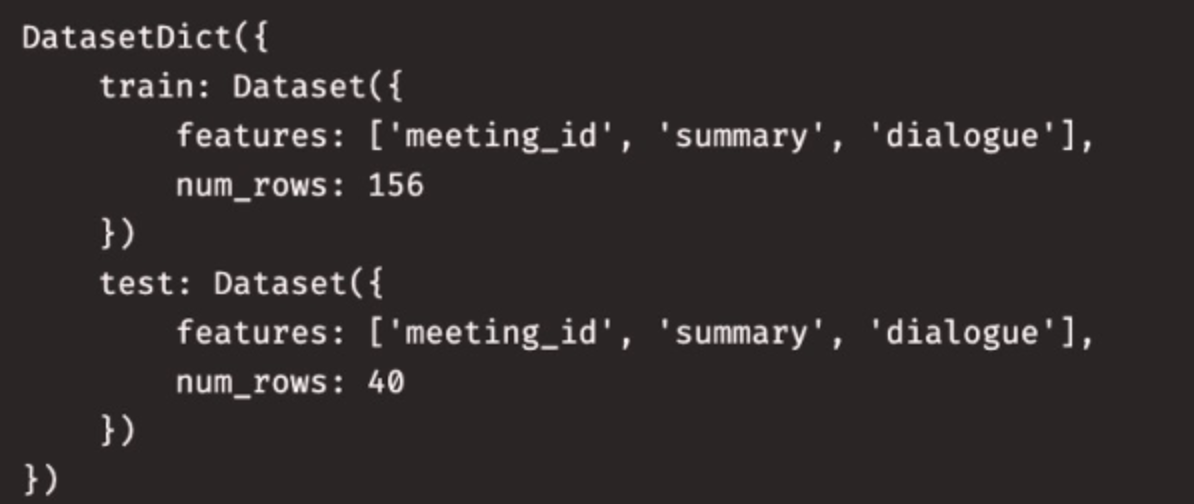
\includegraphics[width=8cm, height=3cm]{figures/JSON}
%	\caption{Example of JSON format}
%	%\Description{autoencoder}
%	\label{fig:TL}
%	\textcolor{red}{Notes: the figure will be replaced with a new TL}
%\end{figure}



\subsection{Quantitative Analysis}

\textcolor{red}{!!! This section needs more work to analyze the results. Any other results for quantitative analysis?}

In this section, we compare two BART models: (1) BART-A: It was trained on the CNN Daily Mail and SAMSUM dataset and retrained the model with our datasets using HuggingFace's Trainer API. This model is suitable for summarizing articles and short chat messages as it was trained. However, it may not produce good summaries for long dialogues \textcolor{red}{[reference?]}. Our quantitative results throughout the epochs are shown in the table below:


%\begin{figure}[thpb]
%	\centering
%	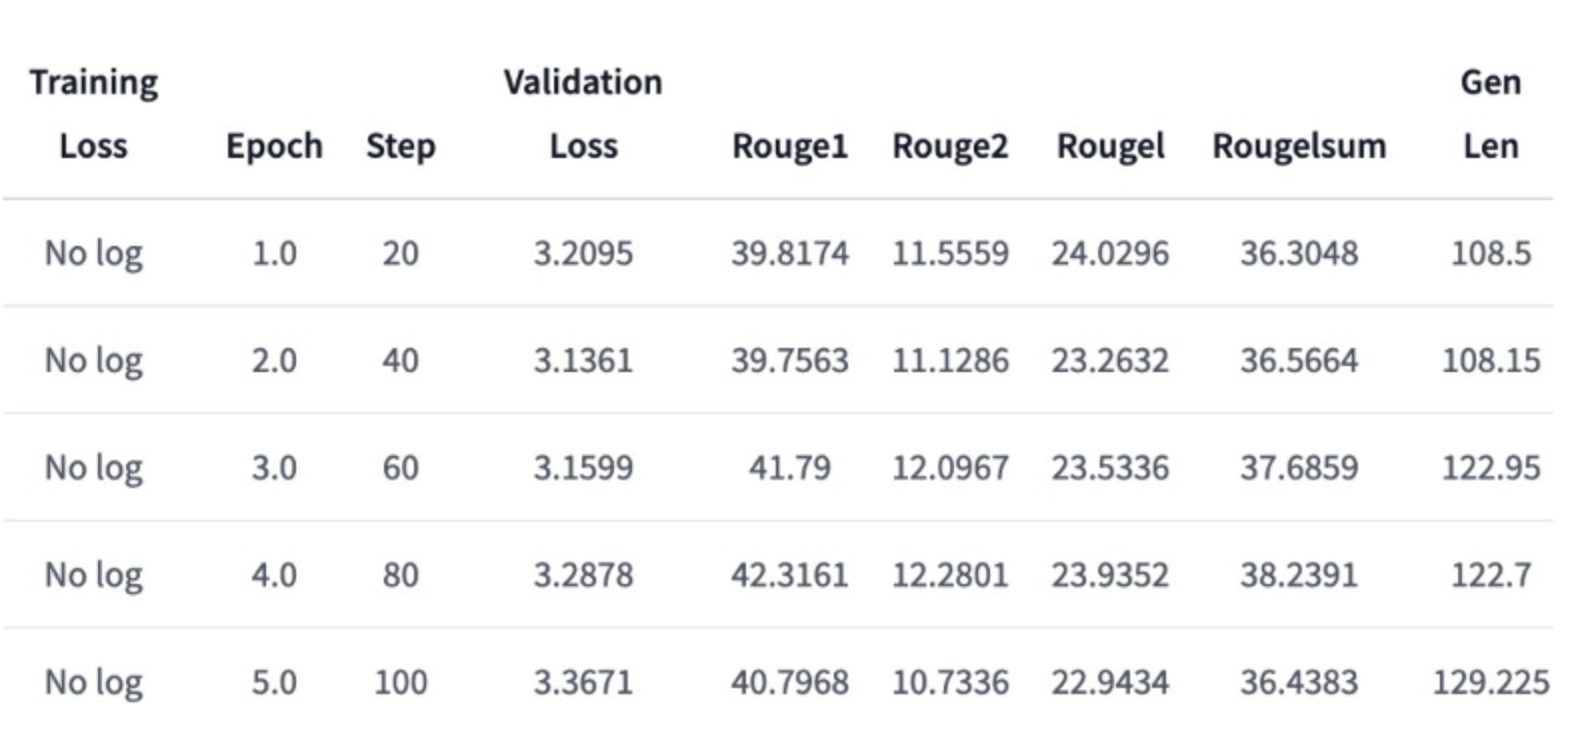
\includegraphics[width=8cm, height=3cm]{figures/res1}
%	\caption{1st model}
%	%\Description{autoencoder}
%	\label{fig:TL}
%	\textcolor{red}{Notes: the figure will be replaced with a table}
%\end{figure}

%
%\begin{table*}[h]
%	\caption{Hyperparameters in model retraining}
%	\label{tab:hyperparam}
%	\begin{center}
%		\begin{tabular}{l|l|l|l|l|l|l|l|l}
%			\hline
%			Epoch & Step & Training loss  & Validation loss & Gen Len & Rouge-1 & Rouge-2 & Rouge-L & Rouge-Lsum \\
%			\hline
%			1 & 20 & No log & 3.2095 & 108.503 & 39.817 & 11.556 & 24.030 & 36.305 \\
%			\hline
%			2 & 40 & No log & 3.1361 & 108.152 & 39.756 & 11.129 & 23.263 & 36.566 \\
%			\hline
%			3 & 60 & No log & 3.1599 & 122.954 &  41.790 & 12.097 & 23.534 & 37.686 \\
%			\hline
%			4 & 80 & No log  & 3.2878 & 122.701 & 42.316 & 12.280 & 23.935 & 38.239 \\
%			\hline
%			5 & 100 & No log & 3.3671 & 129.233 & 40.797 & 10.734 & 22.943 & 36.438 \\
%			\hline
%		\end{tabular}
%	\end{center}
%\end{table*}


\textcolor{red}{What is the difference between Modal-A and Model-B? The second model must have different training, right?}

\textcolor{red}{Need to explain the model performance results}



\begin{table*}[h]
	\caption{Model performance comparison}
	\label{tab:hyperparam}
	\begin{center}
		%\begin{tabular}{l|l|l|l|l|l|l|l|l|l}
			\begin{tabular}{r|r|r|r|r|r|r|r|r|r}
			\hline
			Model & Epoch & Step & Training loss  & Validation loss & Gen Len & Rouge-1 & Rouge-2 & Rouge-L & Rouge-Lsum \\
			\hline
			BART-A & 1 & 20 & No log & 3.2095 & 108.503 & 39.817 & 11.556 & 24.030 & 36.305 \\
			\cline{2-10}
			& 2 & 40 & No log & 3.1361 & 108.152 & 39.756 & 11.129 & 23.263 & 36.566 \\
			\cline{2-10}
			& 3 & 60 & No log & 3.1599 & 122.951 &  41.790 & 12.097 & 23.534 & 37.686 \\
			\cline{2-10}
			& 4 & 80 & No log  & 3.2878 & 122.704 & 42.316 & 12.280 & 23.935 & 38.239 \\
			\cline{2-10}
			& 5 & 100 & No log & 3.3671 & 129.233 & 40.797 & 10.734 & 22.943 & 36.438 \\ 
			\hline
			\hline
				BART-B & 1 & 135 & No log & 3.2308 & 185.794 & 38.427 & 13.646 & 22.366 & 35.235 \\
		\cline{2-10}
		& 2 & 270  & No log & 3.3026 & 146.853 & 40.175 & 11.794 & 23.266 & 36.472 \\
		\cline{2-10}
		& 3 & 405  & No log & 3.5199 & 141.765 & 39.821 & 12.162 & 22.777 & 36.497 \\
		\cline{2-10}
		& 4 & 540  &  2.2131 & 4.0508 & 131.441 & 40.433 & 11.655 & 22.996 & 36.878 \\
		\cline{2-10}
		& 5 & 675  &  2.2131 & 4.6988 & 145.971 & 38.410 & 9.831 & 20.389 & 34.197 \\
		\cline{2-10}
		& 6& 810  &  2.2131 & 4.9590 & 169.245 & 38.576 & 9.634 & 20.865 & 35.032 \\
		\cline{2-10}
		& 7 & 945 & 2.2131 & 5.4264 & 148.039 & 38.281 & 9.576 & 21.141 & 34.599 \\
		\cline{2-10}
		& 8 & 1080 & 0.4010 & 5.4887 & 139.353 & 38.301 & 9.688 & 21.240 & 34.158 \\
		\cline{2-10}
		& 9 & 1215 & 0.4010 & 5.8044 & 145.235 & 39.960 & 10.433 & 22.690 & 36.241 \\
		\cline{2-10}
		&10 & 1350 & 0.4010 & 5.8987 & 138.794 & 39.093 & 10.841 & 21.914 & 35.507 \\
			\hline
		\end{tabular}
	\end{center}
\end{table*}



\begin{table*}[h]
	\caption{Hyperparameters in model retraining}
	\label{tab:hyperparam}
	\begin{center}
				\begin{tabular}{l|l|l|l|l|l|l|l}
							\hline
							Model & learning rate & train batch size & eval batch size &seed & optimizer&LR scheduler type & \# epochs \\
							\hline
							BART-A &  5e-05  &  8 & 8 & 42& Adam, $\beta=(0.9, 0.999), \epsilon=1e-8$& linear & 5 \\
							\hline
							BART-B &  5e-05  &  1 & 1 & 42& Adam, $\beta=(0.9, 0.999), \epsilon=1e-8$& linear & 10 \\
							\hline
						\end{tabular}
			\end{center}
\end{table*}

Table \ref{tab:hyperparam} summarizes hyperparameters we used for the two models. 

%\begin{figure}[thpb]
%	\centering
%	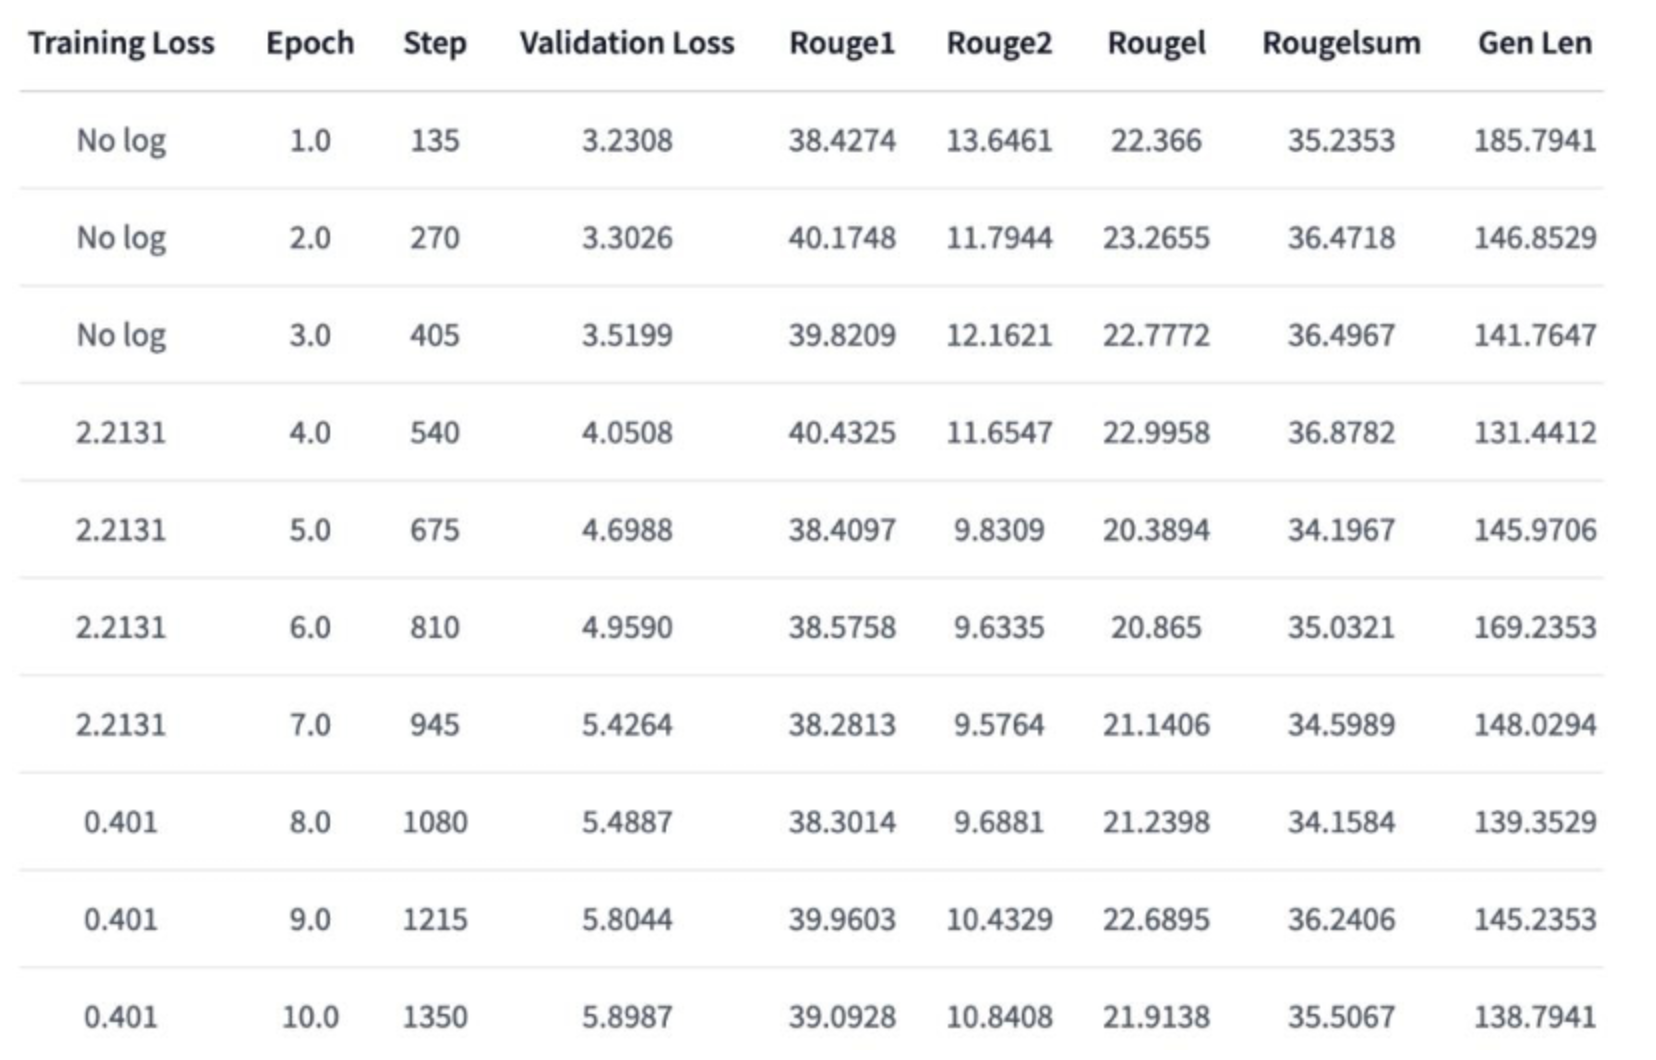
\includegraphics[width=9cm, height=4cm]{figures/res2}
%	\caption{2nd model}
%	%\Description{autoencoder}
%	\label{fig:hyperparam}
%	\textcolor{red}{Notes: the figure will be replaced with a table}
%\end{figure}


\subsection{Qualitative Analysis}

\textcolor{red}{!!! This section needs more work to analyze the results.}

This section presents qualitative results of our proposed pipeline using the BART-B model

We compared to the human reference summary. The output from our model is more comprehensive, accurately identifying the specific locations visited by the individuals. Summaries from BART-B and their corresponding summaries by humans are shown in  Table 3 . 


\begin{table*}[h]
	\caption{Qualitive analysis}
	\label{tab:matrix}
	\begin{center}
				\begin{tabular}{l|l|l}
							\hline
							Type & Machine Summary & Human Reference Summary    \\
							\hline
						Short prose/dialogue & The whole vacation was spent in Paris with my parents. &  \#Person1\# asks Person2\# what \#Person2\# did during  \\
						\textcolor{red}{[ref]}  & 	\textbf{They saw the Eiffel Tower, Nortre-Dame Cathedral, }   & the vacation to Paris.  \#Person2\# saw \textbf{all the most} \\
						&	\textbf{the Seine River, and the famous art museums.} They & \textbf{famous places and enjoyed sitting in cafes most.}  \\
						&	also went a a boat tour around the city, and they had & \#Person1\#'s looking forward a vacation. \\
						&\textbf{a lot of fun sitting in cafes and watching people.}  & \\
							\hline
					Long meeting & This is the \textbf{first meeting of the new remote control}& Manager gave the team members \textbf{a brief introduction} \\
					 \textcolor{red}{[ref]}    & \textbf{project.} Project Manager introduced the team members & \textbf{of the new remote control project}, then the team \\\
					 & to each other and the project manager. The team first  & \textbf{\textcolor{cyan}{started an ice breaking game by drawing their }}  \\
					 & \textbf{\textcolor{cyan}{got acquainted with each other by drawing their}} & \textbf{\textcolor{cyan}{animals. The expected selling price of the remote}} \\
					 & \textbf{\textcolor{cyan}{favourite animals.}} Next, the team discussed the &  \textbf{\textcolor{cyan}{is 25 Euros}} and the production costs would be limited \\
					 & working design of the remote control device. They & to twelve and a half Euro per unit. Marketing plan \\
					 & decided to \textbf{\textcolor{green}{make it more user-friendly}} than the  & would depend on overhead costs. The team agreed that \\
					 & previous one, so they made some changes to the design. & the remote needs to be robust, and they wanted \textbf{\textcolor{green}{it to be}} \\
					 & \textbf{\textcolor{cyan}{The final product would be a remote control with }} & \textbf{\textcolor{green}{a device for all with accessible buttons}}. Project \\
					 & a fancy look, \textbf{\textcolor{green}{ease of use}}, and \textbf{\textcolor{cyan}{cost 25 Euros}}. & Manger suggested it to be only a television remote \\
					 & & control instead of a multi-functional one. \\
					 \hline
					 A meeting of & \multicolumn{2}{l}{Machine Summary (no human reference summary)}\\
					 Load of the Rings & \multicolumn{2}{l}{\textbf{The meeting began with the forging of the Great RINGS, each set with a single GEN, which were given}} \\
					\textcolor{red}{[ref]}   & \multicolumn{2}{l}{\textbf{to the Dwarf Loards, great miners, and craftsmen of the  mountain halls.} Next, the meeting moved onto} \\
					 & \multicolumn{2}{l}{a discussion of the design of the New Line Cinema's next project, which was due to be presented in the next} \\
					 & \multicolumn{2}{l}{meeting. Then, the group moved onto the discussion of how they would govern each other and their own lives. } \\
					 & \multicolumn{2}{l}{\textbf{They discusssed how they could make the best use of the power they had, and decided that they would}} \\
					 & \multicolumn{2}{l}{\textbf{have to be more like the KINGS of Men.} Finally, they talked about how to make the project a success. The} \\
					 & \multicolumn{2}{l}{meeting ended with a brief discussion of their next meeting} \\
					 \hline
						\end{tabular}
			\end{center}
\end{table*}



%\begin{figure}[thpb]
%	\centering
%	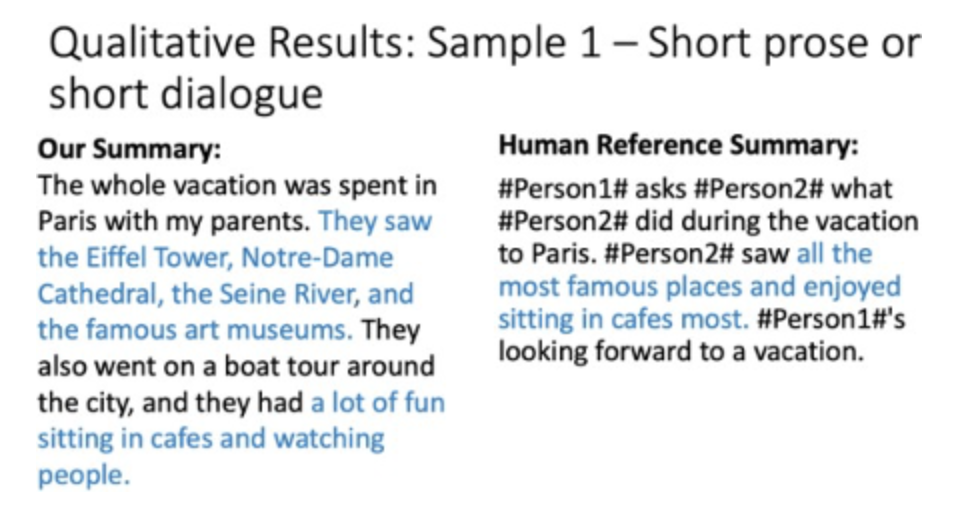
\includegraphics[width=8cm, height=3cm]{figures/q1}
%	\caption{Short prose or dialogue comparison}
%	%\Description{autoencoder}
%	\label{fig:q1}
%	\textcolor{red}{Notes: the figure will be replaced with a table}
%\end{figure}



Our model covers about 60 percent of the content of the reference summary and performs well in most parts. However, in the second sentence, the phrase 'project manager' is unnecessarily repeated at the end.

%
%\begin{figure}[thpb]
%	\centering
%	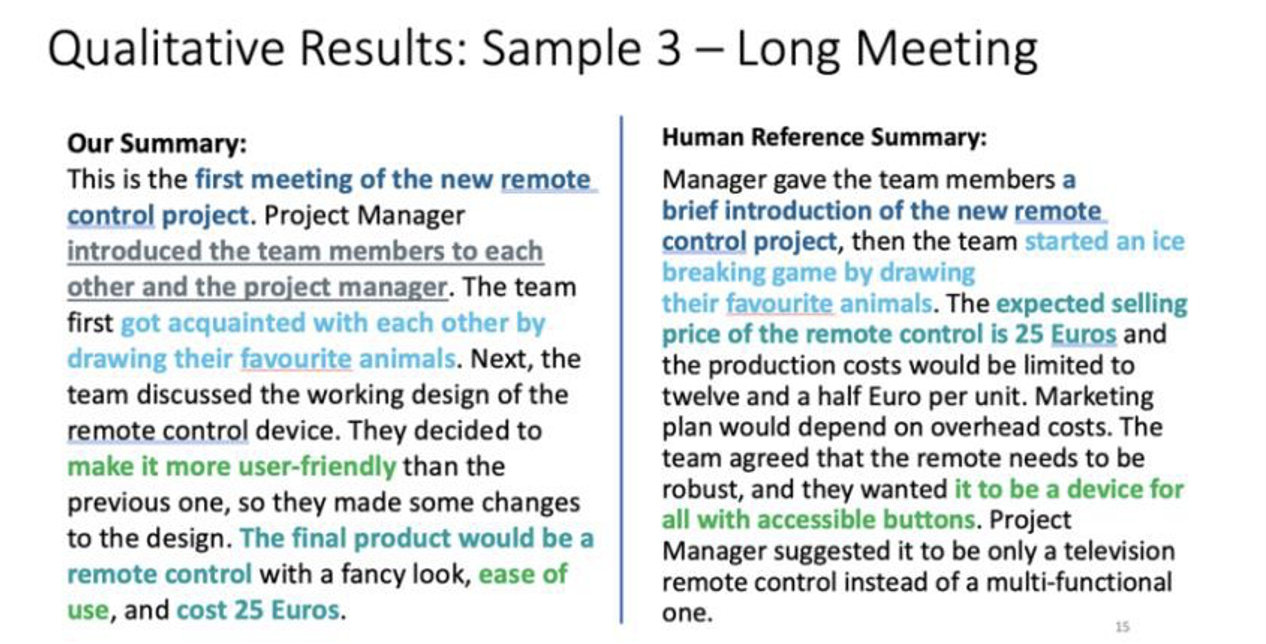
\includegraphics[width=8cm, height=3cm]{figures/q3}
%	\caption{Long meeting summarization comparison}
%	%\Description{autoencoder}
%	\label{fig:q3}
%	\textcolor{red}{Notes: the figure will be replaced with a table}
%\end{figure}







We tested the limits of our model by giving input of the entire Lord of the Rings screenplay to summarize. It has been able to provide a reasonable summary but as one can see it makes a wrong inference that people should be more like the KINGS of Men when they shouldn’t because the KINGS of Men become corrupted by power. We can also see that the model has learned typical workplace lingo such as “The meeting began …” and “They discussed …” due to the transfer learning and finetuning we have carried out.

%\begin{figure}[thpb]
%	\centering
%	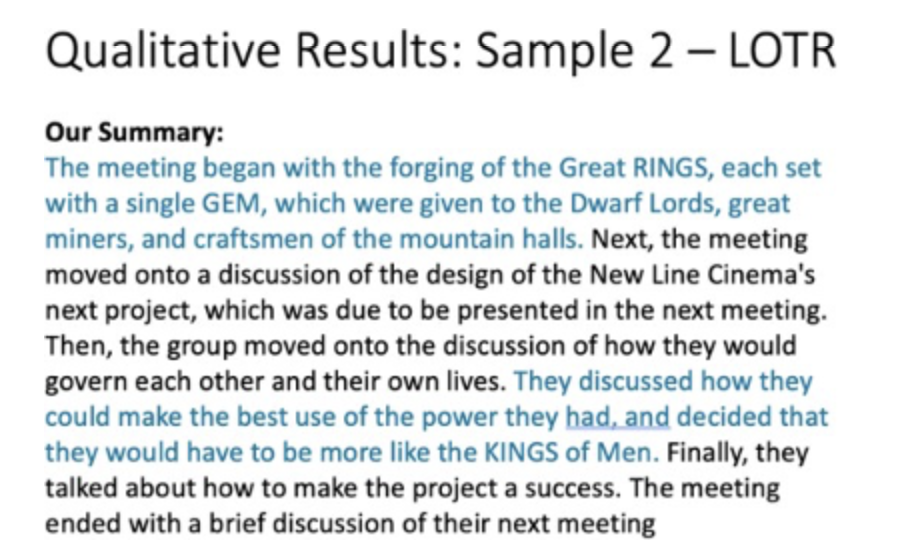
\includegraphics[width=8cm, height=3cm]{figures/q2}
%	\caption{Summarization of Lord of the Rings complete screenplay}
%	%\Description{autoencoder}
%	\label{fig:q2}
%	\textcolor{red}{Notes: the figure will be replaced with a table}
%\end{figure}



%
%\begin{table}[h]
%	\caption{Confusion matrix}
%	\label{tab:matrix}
%	\begin{center}
%			\begin{tabular}{l|l|l|l|l}
%					\hline
%					Metric & IoU Score  & Precision & Recall & F1 Score   \\
%					\hline
%					Average &  0.4111   &  0.555 & 0.856 & 0.710   \\
%					\hline
%				\end{tabular}
%		\end{center}
%\end{table}


%
%\begin{table}[h]
%	\caption{A ligher model for edge computing}
%	\label{tab:matrix}
%	\begin{center}
%		\begin{tabular}{l|l|l|l|l}
%			\hline
%			Model & Classification  & Accuracy & File Size	 & Latency   \\
%			\hline
%			EfficientNet0.tflite&	Pothole	&0.9955	 & 21 MB&	< 15 MS \\
%			&	Normal Road	& & &	 \\
%		\end{tabular}
%	\end{center}
%\end{table}

%\subsection{UI: Django Framework}




%\begin{figure*}[thbp]
%	\begin{center}
%		\mbox{
%			\subfigure[Sensitivity]{
%				\scalebox{0.5}[0.52]{\includegraphics*{figures/real_sen}}
%			}
%			\subfigure[Specificity] {
%				\scalebox{0.5}[0.52]{\includegraphics*{figures/real_spe}}
%			}
%		}
%			\mbox{
%		\subfigure[Precision]{
%			\scalebox{0.5}[0.52]{\includegraphics*{figures/real_pre}}
%		}
%		\subfigure[$F_1$-score] {
%			\scalebox{0.5}[0.52]{\includegraphics*{figures/real_f1}}
%		}
%	}
%		\caption{Performance improvement: LR vs. TL + LR classifiers with 5 SMOTE variants on asthma patients' datasets}
%		\label{fig:zone2}
%	\end{center}
%\end{figure*}
%


%
%\begin{table*}[tphb]
%	\caption{Average model performance of 19 individuals}
%	\label{tab:classification}
%	\begin{center}
%		\begin{tabular}{l|l|cccccc}
%			\hline
%			%\multicolumn{2}{l|}{Algorithm}  & weighted accuracy & sensitivity & specificity & precision & $F_{1}$ score  \\
%			Classifier & Sampling method & weighted accuracy & sensitivity & specificity & precision & $F_{1}$ score  \\
%			\hline
%			\hline
%			DT & \texttt{No up-sampling} & 	0.645& 0.614  &	0.679 &	0.607 &	0.596  \\
%			%\hline 
%			& \texttt{ROS} & 	\textbf{0.738} &	\textbf{0.727} &		\textbf{0.757} &	\textbf{0.687} & \textbf{0.741} \\
%			\hline 
%		\end{tabular}
%		\vspace{2mm}
%		\\ * SMOTE: the synthetic minority over-sampling technique  \cite{chawla2002smote}
%	\end{center}
%\end{table*}

%
%\begin{table*}[tphb]
%	\caption{Classifier performance measures on  asthma patients' datasets}
%	\label{tab:real}
%	\begin{center}
%		\begin{tabular}{l|l|c|cccc|c}
%			\hline
%			%\multicolumn{2}{l|}{Algorithm}  & weighted accuracy & sensitivity & specificity & precision & $F_{1}$ score  \\
%			Classifier & Sampling method & Weighted Acc. & Sensitivity & Specificity & Precision avg. & $F_1$ score avg.  & $S_{rank}$ \\
%			\hline
%			\hline
%			DT & \texttt{No oversampling} &   0.5801 (5) &	0.2780 (7)	&0.8822 (1)	&0.5821	(4) &0.5663 (6) &5.6 \\
%			%\cline{2-7} 
%			& \texttt{ROS} &  0.5779 (6) &	0.3369	(6) &0.8188	(2) &0.5738	(6) &0.5655 (7) &5.8  \\
%			& \texttt{SMOTE} &  0.5813 (5) &	0.3663 (5) &0.7963 (3) 	&0.5727 (6) 	&0.5692 (4)  & 4.8 \\
%			& \texttt{G-SMOTE} &  0.5851 (3)	&0.3781	(4) &0.7880 (6) 	&0.5838 (3) 	&0.5697 (3) & 3.8 \\
%			%& \texttt{ACOR-SMOTE} &  0.5977	&0.4790	&0.7165	&0.5761	&0.5648 \\
%			& \texttt{Gamma-SMOTE} &  0.5849 (4) &	0.3901 (2) &0.7797 (7)	&0.5798 (5)	&0.5677 (5) & 3.7  \\
%			& \texttt{SDD-SMOTE} &  0.5955 (1)	&0.3980 (1) &	0.7931 (5)	&0.5850	(2) &0.5773 (2)  & \textbf{1.8} \\
%			& \texttt{$^{*}$ANVO} &  0.5873	(2) &0.3803 (3) &	0.7944 (4) &	0.5891 (1) &0.5776 (1) & \textbf{2.3} \\			
%			\hline 
%			KNN & \texttt{No oversampling} & 	0.5443 (7)	&0.1279 (7)	&0.9607	(1) &0.5575	(7) &0.5195 (7)   &6.4\\
%			%\cline{2-7} 
%			& \texttt{ROS} & 0.5996	(5) &0.4742	(6) &0.7250	(2) &0.5792	(3) &0.5734 (1) &4.0\\
%			& \texttt{SMOTE} &  0.6188	(1) &0.5697	(1) &0.6679	(5) &0.5829	(1) &0.5673 (2) & \textbf{1.6} \\
%			& \texttt{G-SMOTE} &  0.6067 (2) &	0.5441	(3) &0.6692	(4) &0.5798	(2) &0.5635 (3) & \textbf{2.9}  \\
%			& \texttt{Gamma-SMOTE} &  0.5902 (6) 	&0.5262	(5) &0.6541	(7) &0.5666	(6) &0.5452 (6) & 5.6\\
%			& \texttt{SDD-SMOTE} &  0.6061	(3) &0.5500	(3) &0.6623	(6) &0.5783	(4) &0.5615 (4) & 3.7 \\
%			& \texttt{$^{*}$ANVO} &  0.6025	(4) &0.5601 (2) &0.6731	(3) &0.5768	(5) &0.5608  (5) & \textbf{3.3} \\			
%			\hline 
%			LR & \texttt{No oversampling} & 	0.5303 (7)	&0.0762	(7) &0.9844	(1) &0.4656	(7) &0.4864 (7) & 6.4 \\
%			& \texttt{ROS} &  0.6088 (6) &	0.5175 (5) &0.7002 (7)	&0.5716 (6) &0.5606 (6) &5.1 \\
%			& \texttt{SMOTE} &  0.6168 (5)	&0.5028 (6) &0.7308	(4) &0.5933 (3)	&0.5852 (2) &4.4 \\
%			& \texttt{G-SMOTE} &  0.6199 (3)	&0.5260	(3) &0.7338	(2) &0.5992 (1)	&0.5884 (1)  & \textbf{2.1} \\
%			& \texttt{Gamma-SMOTE} &  0.6215 (2) &	0.5195 (4) 	&0.7134 (5)	&0.5918 (4) 	&0.5812  (4) & 4.1 \\
%			& \texttt{SDD-SMOTE} &  0.6240 (1)	&0.5390 (1)	&0.7089 (6) &0.5894 (5) 	&0.5805 (5) & \textbf{3.1} \\
%			& \texttt{$^{*}$ANVO} &  0.6194 (4)	&0.5301 (2) &0.7315 (3)	&0.5971	(2)&0.5847 (3)  & \textbf{2.3} \\			
%			\hline 
%			NB & \texttt{No oversampling} & 	0.5383 (7)	&0.0987 (7)	&0.9778 (1)	&0.5024 (7)	&0.5019 (7) & 6.4  \\
%			%\cline{2-7} 
%			& \texttt{ROS} & 0.6072 (1) 	&0.5096	(1) &0.7048	(7) &0.5714	(6) &0.5608 (6) & 3.6 \\
%			& \texttt{SMOTE} &  0.5992 (4) 	&0.3783	 (5) &0.8201 (2)	&0.5995	(2) &0.5910  (1) & \textbf{3.3} \\
%			& \texttt{G-SMOTE} &  0.5935 (5)	&0.3921	(3) &0.7948	(6) &0.5880	(3) &0.5823 (3) & \textbf{3.3} \\
%			& \texttt{Gamma-SMOTE} & 0.5892 (6) 	&0.3761	(6) &0.8023	(5) &0.5838	(5) &0.5753 (5) & 5.5 \\
%			& \texttt{SDD-SMOTE} &  0.6011	(3) &0.3880	(4) &0.8141	(3) &0.6016	(1) &0.5876 (2) & \textbf{2.9} \\
%			& \texttt{$^{*}$ANVO} &  0.6028	(2) &0.3952	(2) &0.8103	(4) &0.5843	(4) &0.5822 (4) & \textbf{3.0}  \\			
%			\hline 
%		\end{tabular}
%		\vspace{2mm}
%		\\ *  indicates our new SMOTE variant. 
%	\end{center}
%\end{table*}
%

